\section{Genomic combination}

\subsection{Sanger assembly: overlap-layout-consensus algorithm}

We can think about the reads as the potential vertexes that we 
want to connect with edges. 
So \textbf{we want to find the edges connecting our reads}.
The sequence-overlaps between reads will allow us to define the 
edges of our Hamiltonian path.  
So it is possible to build the path with simple greedy algorithms
without the need to calculate all the possible hamiltonian paths to 
find the best fit.
If we have n reads, we will need to calculate $n^2$ possible overlaps.\\

With the sanger assembly we have to:
\begin{enumerate}
  \item calculate pairwise alignments of all fragments
  \item choose two fragments with the largest overlap
  \item merge chosen fragments
  \item repeat setp 2 and 3 until only one fragment is left
\end{enumerate}

The problem with this approach is that it takes a lot of time (the complexity
is exponential). How can we solve this problem?\\

\subsection{Shotgun fragmentation and assembly}

Consider this minute single stranded DNA circular genome, 14 bases long.
Random fragments can start from any of the 14 positions.
We can imagine to produce reads of just 3 bases, considering that the
reads included in repeats will be found at a higher rate.

\begin{figure}[H]
  \centering
  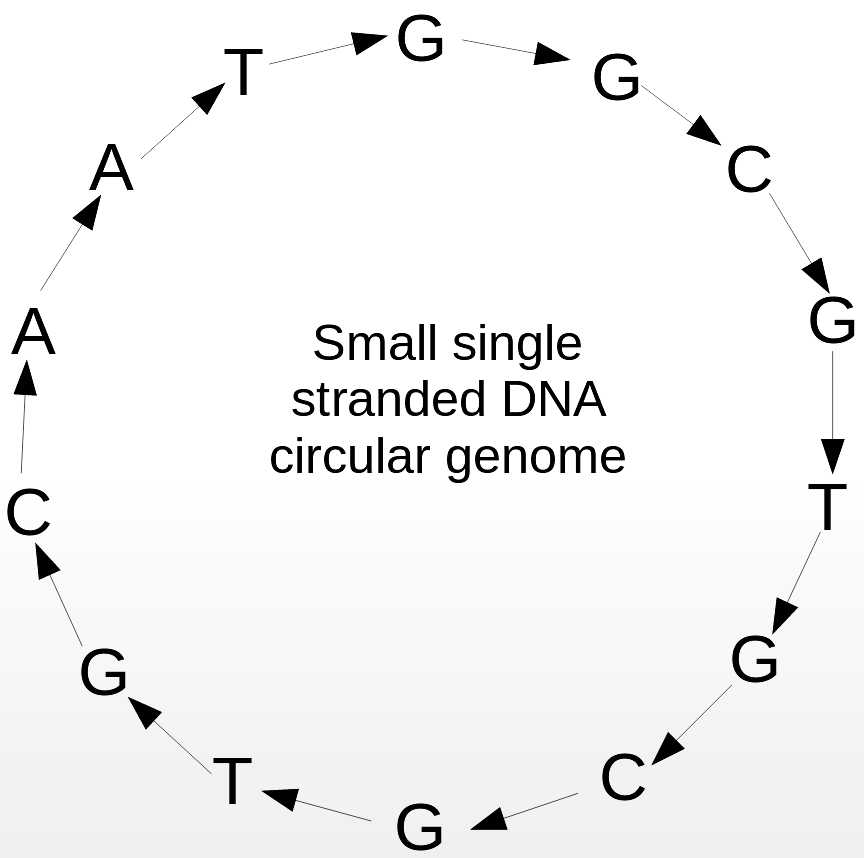
\includegraphics[scale=0.25]{smalldna}
  \caption{example dna}
  \label{fig:smalldna}
\end{figure}

The reads are:

\texttt{GGC, GCG, CGT, GTG, TGC, GCG, CGT, GTG, TGC, GCA, CAA, AAT, ATG, TGG}

Classic methods for de novo assembly are based on connecting reads by overlaps.\\
 
\textbf{reads $=$ graph nodes}
 
\textbf{overlaps $=$ edges}\\

Since there may be repeats, the graph may not be linear. 
The assembly algorithm must find the most plausible path in the graph.

\begin{figure}[H]
  \centering
  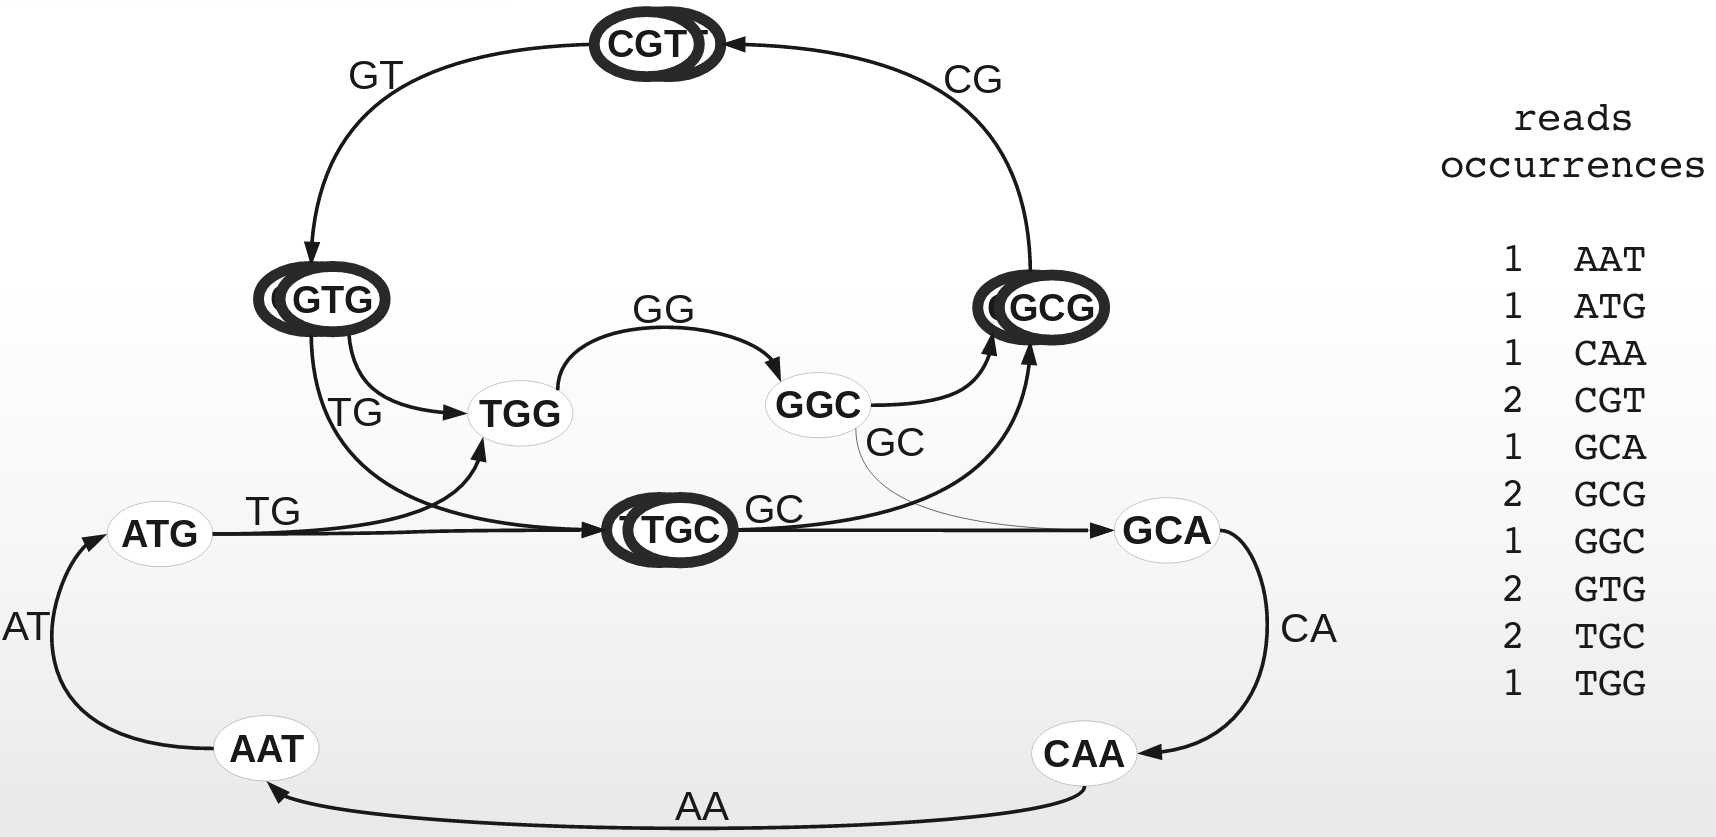
\includegraphics[scale=0.25]{graphreads}
  \caption{graph with reads and occurences}
  \label{fig:graphreads}
\end{figure}

In our graph (figure \ref{fig:graphreads}) we should find a path 
going over each node only once.

Some sequences occurring at a higher rate may be repeated more 
than once (bold circles) and we could represent them by two or more nodes
with the same sequence. 

Finding a path in a graph, passing \textbf{once over each node}, is known as
Hamiltonian path problem.

A Hamiltonian cycle is a Hamiltonian path that starts and ends at the same point.

This lead to the \textit{Hamiltonian Problem}, that is a
very difficult problem (NP-hard)

Another solution is to implement an Eulerian path, that goes
\textbf{once over each edge}, and it's a simpler problem.

In the specific case of sequence assembly, an  Eulerian path can be
obtained by considering the reads as edges and the overlaps as vertices.

\begin{figure}[H]
  \centering
  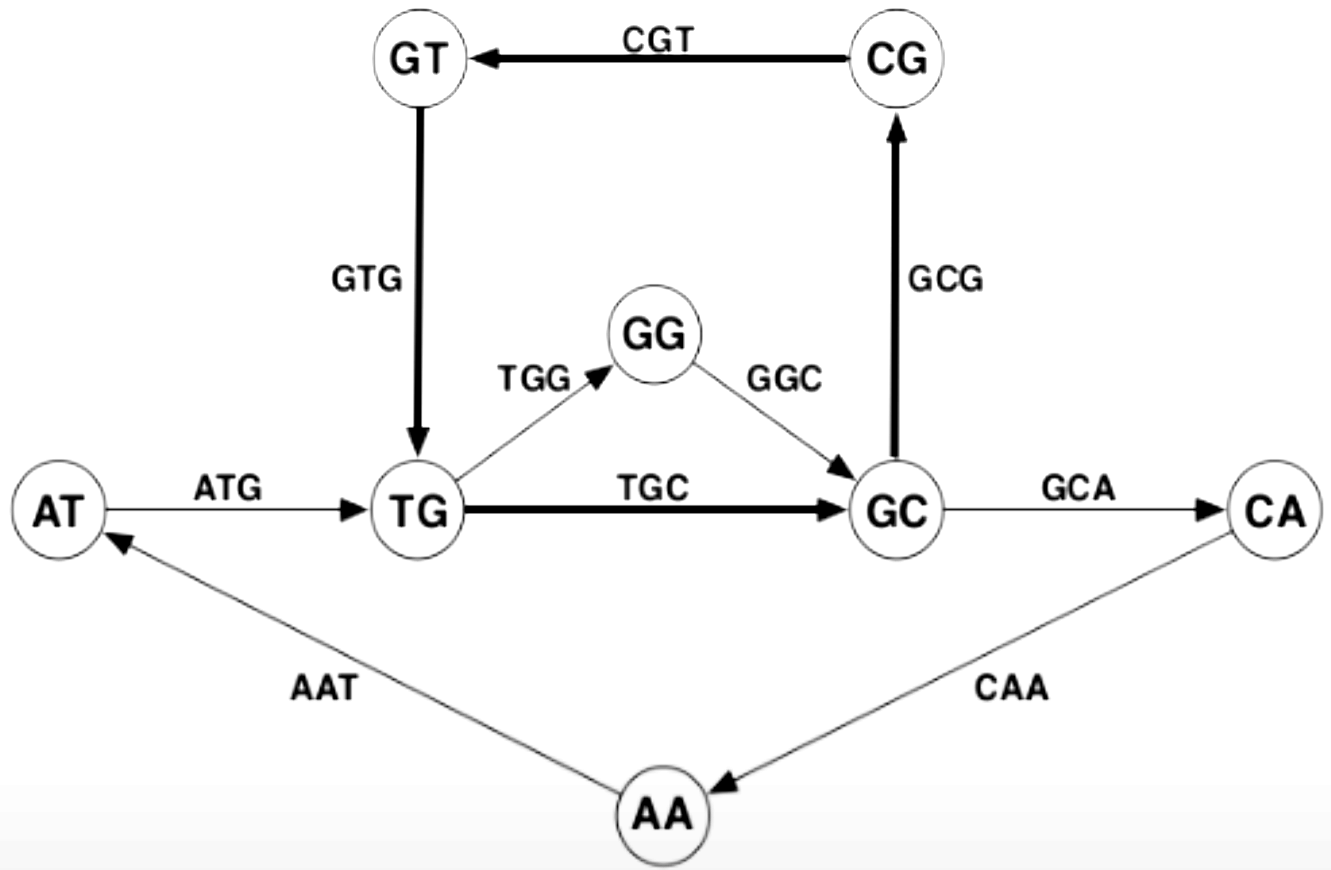
\includegraphics[scale=0.25]{eulerianreads}
  \caption{graph with reads as edges}
  \label{fig:eulerianreads}
\end{figure}

Also in this case we want to walk once over each read, but 
now the reads are edges instead than vertices.

\textbf{Computationally the two problems are very different}.

The Eulerian solution doesn't solve the problem of overlaps.

\subsubsection{Be Bruijn graphs and Eulerian path}
This is the best solution for now, and use a study published by the
matematician Be Bruijn.
Steps for the solution:
\begin{enumerate}
  \item In pratical terms, a shotgun library is made and it is sequenced at a
reasonably high coverage, for instance 60x
  \item The resulting fastq file is read once, and all the kmers are counted.
This process will produce a list of all the kmers and their frequency
  \item We can start from any kmer that was found at the expected frequency and
we can extend the resulting conting by moving one position at a time. At every
step we will need to choose one of the 4 possible kmers. This will be done by
looking at the list of kmers. If there are no repeats then only one of the four
kmers should be present in the list.
\end{enumerate}

What is the best lenght of kamers to have the best use? What happens with long
kmers?
